
\documentclass[letterpaper,11pt]{article}
\usepackage{latexsym}
\usepackage{enumitem}
\usepackage{mathtools}
\usepackage{amsmath}
\usepackage[empty]{fullpage}
\usepackage[usenames,dvipsnames]{color}
\usepackage{verbatim}
\usepackage{xcolor}
\usepackage[colorlinks = true,
linkcolor = red,
urlcolor  = red,
citecolor = red,
anchorcolor = red]{hyperref}

\newcommand{\MYhref}[3][red]{\href{#2}{\color{#1}{#3}}}%
%\usepackage[pdftex]{hyperref}

%\hypersetup	{
%			    colorlinks,
%			    citecolor=black,
%			    filecolor=black,
%			    linkcolor=black,
%			    urlcolor=black 
%			}
\definecolor{mygrey}{gray}{.85}
\definecolor{mygreylink}{gray}{.40}
\textheight=9.0in
\raggedbottom
\raggedright
\setlength{\tabcolsep}{0in}

% Adjust margins
\addtolength{\oddsidemargin}{-0.375in}
\addtolength{\evensidemargin}{0.375in}
\addtolength{\textwidth}{0.5in}
\addtolength{\topmargin}{-.375in}
\addtolength{\textheight}{0.75in}
\newlength{\arrow}
\settowidth{\arrow}{\scriptsize$100000$}
\newcommand*{\myrightarrow}[1]{\xrightarrow{\mathmakebox[\arrow]{#1}}}

%Custom commands
\newcommand{\resitem}[1]{\item #1 \vspace{-2pt}}
\newcommand{\resheading}[1]{{\large \colorbox{mygrey}{\begin{minipage}{\textwidth}{\textbf{#1 \vphantom{p\^{E}}}}\end{minipage}}}}
\newcommand{\ressubheading}[4]{
\begin{tabular*}{6.5in}{l@{\extracolsep{\fill}}r}
		\textbf{#1} & #2 \\
		\textit{#3} & \textit{#4} \\
\end{tabular*}\vspace{-6pt}}

\newcommand{\ressubsubheading}[2]{
\begin{tabular*}{6.5in}{l@{\extracolsep{\fill}}r}
		\textit{#1} & \textit{#2} \\
\end{tabular*}\vspace{-6pt}}

\begin{document}
% Center the name over the entire width of resume:
{\LARGE\bf You Zhou}{$\,\,$\MYhref{mailto:kecen.zhou@gmail.com}{kecen.zhou@gmail.com}}
\vspace{0.2in}\\
%\resheading{Diagram}
%\\$\,$\\$\,$\\
%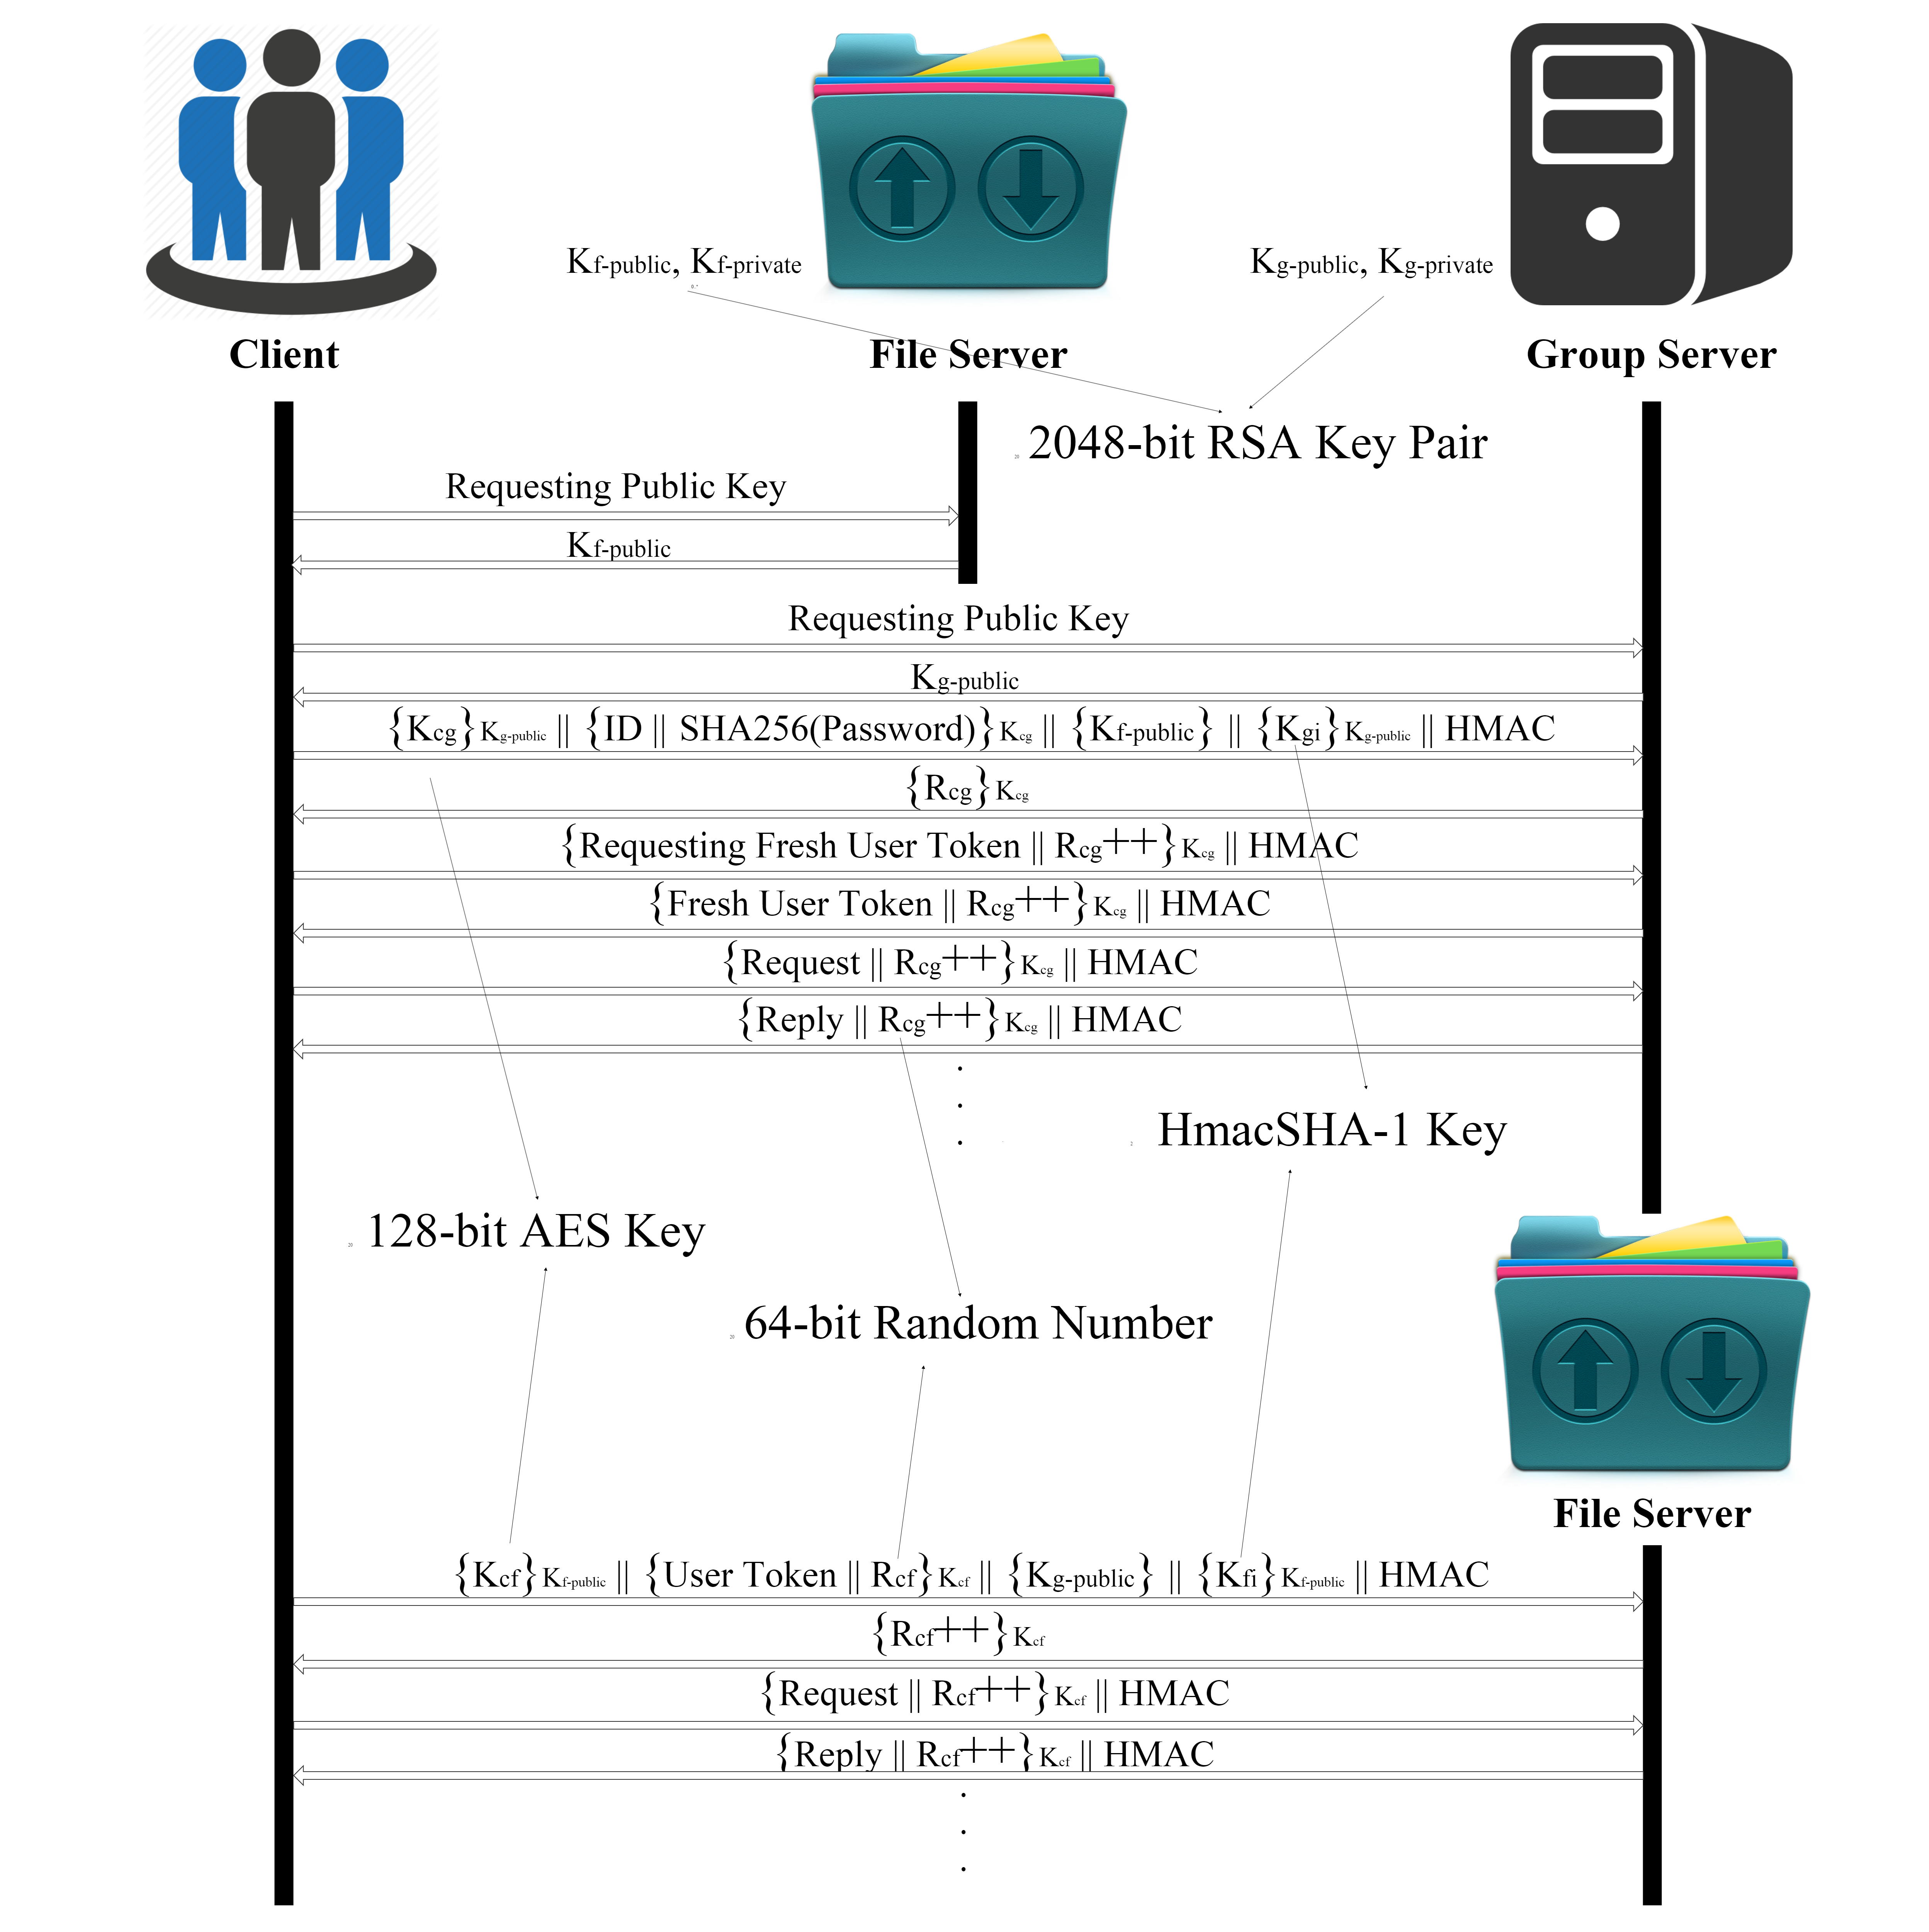
\includegraphics[scale=0.108]{protocols}
%\\$\,$\\$\,$\\
%\resheading{Introduction}
 %      \begin{flushleft}
%			$\,\,\,\,\,\,\,\,\,\,\,\,\,\,\,\,\,\,$In this last phase, the designing features of authorizations as well as the network protocols will be scrutinized further in the position of an attacker.   
 %       \end{flushleft}
  %      \vspace{0.2in}
\resheading{AuthInfo Leakage (Implemented)}
\vspace{0.1in}
\begin{itemize}[noitemsep,topsep=0pt,parsep=1pt,partopsep=1pt]
	\item\textbf{Threat Description}
	\begin{flushleft}
		In this phase, assumption made upon group server that it will never be compromised will be weakened to a degree that its passwords field holding $<\textrm{ID, SHA256(passwords)}>$ is at the risk of leaking out, and when it happens, dictionary attacks are almost definitely followed. Considering most users are bad passwords choosers, by online hash cracking engine like \MYhref{http://www.hashhunters.net/}{Hash Hunters}, naive passwords such as ``baseball'' and ``basketball'' can be figured out immediately. Worse, as the number of users climbs up, the chances of having two users with the same passwords become concerning, meaning that by cracking one, attackers actually crack down two or more. 
	\end{flushleft}
	\item\textbf{Mechanisms}
	\begin{flushleft}
		By concatenating a random 
	\end{flushleft}
\end{itemize}
	%\item\textbf{Mechanism}
		%\begin{flushleft}
			%Another choice for an unforgeable and verifiable ADMIN identity is letting group server sign the name ADMIN with its private key and save the result as the group name instead.  
		%\end{flushleft}
		%\begin{flushleft}
		%	Users are expected to be very active during his/her session, so communication should not be secured by RSA for its inefficiency. However, the group server still needs a 1024-bit RSA key pair $<K_{gs},\,K_{gs}^{-1}>$ to exchange a 128-bit AES key $K_{cg}$ per session. Indeed, 3DES also maintains a good security level but applying AES once is probably more efficient (elegant) than applying DES three times -- DES is not software friendly in nature. The operation mode chosen for AES is CTR because first it only takes XOR for encryption/decryption, and second its IV can be generated in advance. The most lethal AES setting to avoid is not to use the same IV to encrypt any two messages within the same session! An attacker can get XORed byte array of two messages by simply XORing their corresponding cipher texts. To minimize the chance of IV collision, IV will be 128-bit(16-byte) in length.
		%\end{flushleft}
		%\vspace{0.25in}
		%$\,\,\,\,\,\,\,\,\,\,\,\,\,\,\,\,\,\,\,\,\,\,\,\,\,\,$
		%\setlength{\tabcolsep}{10pt}
		%\begin{tabular}{ccc}
			%
\includegraphics[width=3cm,keepaspectratio]{c} & 
			%\raisebox{5ex}{%
			%\begin{tabular}{c}
			%	$\underrightarrow{\quad\,\,\,\,\,\,\,\,\,\,\,\,\,\,\,\,\,\,\,\,\,\,\,\,\,\,\,\,1.\left\lbrace R\,||\,K_{cg}\right\rbrace_{K_{gs}}\,\,\,\,\,\,\,\,\,\,\,\,\,\,\,\,\,\,\,\,\,\,\,\,\,\,\,\,\quad}$\\
				%$\underleftarrow{\quad\,\,\,\,\,\,\,\,\,\,\,\,\,\,\,\,\,\,\,\,\,\,\,\,\,\,\,\,\,\,\,2.\left\lbrace R-1\right\rbrace_{K_{cg}}\,\,\,\,\,\,\,\,\,\,\,\,\,\,\,\,\,\,\,\,\,\,\,\,\,\,\,\,\,\,\,\quad}$\\
				%$\underrightarrow{\quad3.\left\lbrace \textrm{user\_name}\,||\,\textrm{SHA-1(password)}\right\rbrace_{K_{cg}}\quad}$\\
				%$\underleftarrow{\quad\,\,\,\,\,\,\,\,\,\,\,\,\,\,\,\,\,\,\,\,\,\,\,\,\,4.\left\lbrace\textrm{user\_token}\right\rbrace_{K_{cg}}\,\,\,\,\,\,\,\,\,\,\,\,\,\,\,\,\,\,\,\,\,\,\,\,\,\quad}$\\$\,$\\$\,$\\$\,$\\
			%\end{tabular}} &
			%
\includegraphics[width=3cm,scale=0.7]{s}
		%\end{tabular}
	%\begin{flushleft}
	%	Password is not transmitted or stored in plain text to prevent leakage when the group server is compromised. Because the most recent MD version MD5 was broken in 2008, SHA-1 is used instead to digest password. 
	%\end{flushleft}
	%\begin{flushleft}
	%	The identity of the group server will be authenticated as soon as it replies $\{R-1\}_{K_{cg}}$. Group client after decryption will be convinced that the group server really owns the private key $K_{gs}^{-1}$. To authenticate the group client, the group server checks the received password digestion against the one its saved in its database. In addition to issuing token, the group server will also generate a signature on token, and this operation will be discussed in the following section. 
	%\end{flushleft}
	%\item\textbf{Correctness/Security}
	%\begin{flushleft}
	 %The shared symmetric session key $K_{cg}$ that both client and server agree upon ensured the correctness of message being transmitting. RSA encryption/decryption used during the initial key exchange secures the later communication for it prevents any third party from knowing $K_{cg}$.    
	%\end{flushleft}
%\end{itemize}
\vspace{0.1in}

\resheading{T2 File Key Leakage}
\vspace{0.1in}
\begin{itemize}[noitemsep,topsep=0pt,parsep=1pt,partopsep=1pt]
	\item\textbf{Threat Description}
	\begin{flushleft}
		A per group file key list is stored in the group server, but the list is stored unencrypted. Attackers are assumed to be very efficient to steal the encrypted files from file servers, so the associated file keys are the final defend against them. Once the group server is compromised, the confidentiality of files would be no longer ensured.       
	\end{flushleft}
	\item\textbf{Mechanism}
	\begin{flushleft}
		The group server will generate a per group master key to encrypt the file key list object, and the master key will be exported to each member of the group in binary format. Every time before a download request, group members need to import the binary file to the group server first so that the restored master key can decrypt the file key object. 
	\end{flushleft}
	%$\,\,\,\,\,\,\,\,\,\,\,\,\,\,\,\,\,\,\,\,\,\,\,\,\,\,$
	%\setlength{\tabcolsep}{10pt}
	%\begin{tabular}{ccc}
	%	
\includegraphics[width=3cm,keepaspectratio]{c} & 
	%	\raisebox{5ex}{%
	%		\begin{tabular}{c}
	%			$\underrightarrow{\quad\,\,\,\,\,\,\,\,\,\,\,\,\,\,\,\,\,\,\,\,\,\,\,\,\,\,\,\,1.\left\lbrace R\,||\,K_{cf}\right\rbrace_{K_{fs}}\,\,\,\,\,\,\,\,\,\,\,\,\,\,\,\,\,\,\,\,\,\,\,\,\,\,\,\,\quad}$\\
				%$\underleftarrow{\quad\,\,\,\,\,\,\,\,\,\,\,\,\,\,\,\,\,\,\,\,\,\,\,\,\,\,\,\,\,\,\,2.\left\lbrace R-1\right\rbrace_{K_{cf}}\,\,\,\,\,\,\,\,\,\,\,\,\,\,\,\,\,\,\,\,\,\,\,\,\,\,\,\,\,\,\,\quad}$\\
				%$\underrightarrow{\,\,\,\,\,\,\,\,\,\,\,\,\,\,\,\,\,\,\,\,\,\,\,\quad3.\left\lbrace\textrm{user\_token}\right\rbrace_{K_{cf}}\,\,\,\,\,\,\,\,\,\,\,\,\,\,\,\,\,\,\,\,\,\,\,\,\,\,\quad}$\\
				%$\,$\\$\,$\\			
			%\end{tabular}} &
			%
\includegraphics[width=3cm,scale=1.1]{f}
		%\end{tabular}
	%\begin{flushleft}
		%The first two steps are basically the same as for the last section. The file client checks file server's identity by decrypting $\left\lbrace R-1\right\rbrace_{K_{cf}}$. The file server will not signal whether a received token is valid or not after step 3, since the file client will learn it by listing accessible files after operation.
	%\end{flushleft}
	%	\item\textbf{Correctness/Security}
		%\begin{flushleft}
		%	 The correctness of the token verification relies mainly on the signature signed by the group server that is assumed trustworthy and will not be compromised. The correct communication between file client and file server depends on the shared key $K_{fs}$ that is exchanged in a RSA secured manner just as the case in the last section.   
		%\end{flushleft}
	\end{itemize}
    \vspace{0.1in}
    
    \resheading{Threat 3: File Key Non-Renewal }
    \vspace{0.1in}
    \begin{itemize}[noitemsep,topsep=0pt,parsep=1pt,partopsep=1pt]
    	\item\textbf{Threat Description}
    	\begin{flushleft}
			In the current setting, files live forever with the file keys used to upload them. However, the longer the file key stays unchanged, the more likely it would be learned by attackers.    
    	\end{flushleft}
    	\item\textbf{Mechanism}
    	\begin{flushleft}
			Since we generate a new file key every time a group member is revoked, the key list object tends to hold a huge number of keys as the time goes. For renewal process, generating a new key to substitute all keys existing is impractical because encrypted files need to be decrypted first with their associated old keys and then encrypted with the new key -- it is time costly. Hence, the renewal mechanism will only target files requested most often, since the more often they are requested, the more features of them can be learned by attackers.      
    	\end{flushleft}
    		%\item\textbf{Correctness/Security}
    		%\begin{flushleft}
			%	The correctness relies on client's knowledge of file server's public key $K_{fs}$ and file server's exclusive knowledge of the private key $K_{fs}^{-1}$. These two requirements are ensured by assumptions. Moreover, RSA also ensures the security by the security of itself. 
    		%\end{flushleft}
    	\end{itemize}
    	\newpage
        \resheading{Threat 4: DoS Attack}
        \vspace{0.1in}
        \begin{itemize}[noitemsep,topsep=0pt,parsep=1pt,partopsep=1pt]
        	\item\textbf{Threat Description}
        	\begin{flushleft}
				%Encrypted messages, especially the repeated ones, can provide information of the plain texts to passive attacker who is monitoring. For example, when ADMIN creates lots of users at the beginning of his/her session, a steady stream of encrypted message ``CUSER'' would be observed by passive attacker, and as a result, he/she would know a new user has been created whenever the cipher text of ``CUSER'' is observed.
				Attackers can easily spawn huge number of threads requesting handshaking process or other operations repeatedly to paralyze the servers. Legitimate clients in that scenario will not be able to access to or receive reply from servers.  
        	\end{flushleft}
        	\item\textbf{Mechanism}
        	\begin{flushleft}
        		%Mechanisms implemented for both T1 and T2 already avoided any message to be sent in plain text, and the encryption by the 128-bit AES/CTR has been randomized so that any message will be encrypted into different cipher texts each time. This is achieved by generating IV of the CTR operation per operation. The collision is unlikely to happen because of the 128-bit length of the IV.
        		Servers will put a certain limit on the amount of requests can be sent from each IP address per unit time. For specific operations: 1.handshaking requests will be only allowed to do twice per login. 2.upload/download the same files will only be allowed to do twice per day. 3.group creation can only be requested three times per day. 4.deleting groups that are not existing for three times will result immediate disconnection.      
        	\end{flushleft}
        	%\item\textbf{Correctness/Security}
        	%\begin{flushleft}
			%	The correctness and the security of this mechanism have been discussed during the last three sections. They basically rely on the correct implementation of the chosen cipher. 
        	%\end{flushleft}
        \end{itemize}
        %\vspace{0.2in}
        %\resheading{Conclusion}
        %\begin{flushleft}
        %	%SAM YOU FILL THIS.
        %\end{flushleft}
\end{document}
